\documentclass[handout]{ximera}


\input{../preamble}

\outcome{Estimate limits using numerical information}

\title{1.2 Numerical Limits}

\begin{document}

\begin{abstract}
We find limits using numerical information.
\end{abstract}

\maketitle


\section{Limit notation}

Limits are the backbone of calculus. A limit tells us the end of an infinite process. For example, consider the following infinite sequence of numbers:
\[ 0.9, 0.99, 0.999, 0.9999, 0.99999, 0.999999, ... \]
This infinite sequence of numbers is becoming arbitrarily close to the number 1, so we say the \textbf{limit} of the sequence is 1.
In calculus, we will be concerned with limits involving functions.
%A function is an input-output device involving numbers. 
The inputs of the function will undergo an infinite process which will then correspond to an infinite process for the outputs.  
Our goal will be to determine the limit of the outputs.
Suppose that $f$ represents a function of the input variable $x$.
We denote by $x \to c$ an infinite process where the inputs are becoming arbitrarily close to the value $c$ without ever reaching it.
Then, we denote by
\[ \lim_{x\to c} f(x) \]
the limit of the outputs of the function $f$ as $x$ approaches $c$.
The possibilities for the limit of the outputs of $f$ are: a numerical value, 
$\infty$, $-\infty$, or that the limit does not exist.
If the numerical value of the limit is $L$, then as the input variable $x$ approaches the value $c$, the outputs, $f(x)$ approach the value $L$, and we would write

\[ 
\lim_{x\to c} f(x) = L
\]

If the value of the limit is $\infty$, then as $x \to c$, the outputs $f(x)$ are \textbf{increasing without bound},
and we write
\[
\lim_{x \to c} f(x) = \infty
\]
  
Similarly, if the limit is $-\infty$, that means the outputs are decreasing without bound, and we write
\[
\lim_{x \to c} f(x) = -\infty
\]

If none of the previous conclusions apply, we say that the limit \textbf{does not exist}, and we write
\[
\lim_{x \to c} f(x) \;\; \text{DNE}.
\] 

In addition to writing $x \to c$, we can also write the expression
$x \to c^-$ to indicate that $x$ is approaching $c$ from the left-hand side and $x \to c^+$ to 
indicate that $x$ is approaching $c$ from the right-hand side.

The expression $x \to c^-$ can be understood visually using the following diagram:




\begin{center}
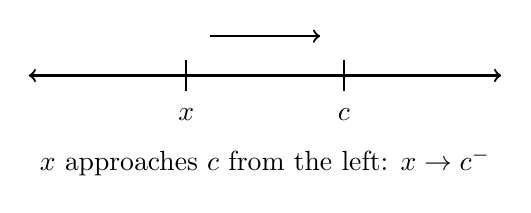
\begin{tikzpicture}
\draw[<->, thick] (-3,0) -- (3,0);
\draw[thick] (-1,-.2) -- (-1,.2); %tick mark
\draw[thick] (1,-.2) -- (1,.2);
\node[below] at (-1,-.3) {$x$};
\node[below] at (1,-.3) {$c$};
\draw[->, thick] (-0.7,0.5) -- (0.7,0.5);
\draw[white](0, .6) -- (.1, .6);
\node[below] at (0,-0.8) {$x$ approaches $c$ from the left: $x \to c^-$};


\end{tikzpicture}

\end{center}

Note that $x \to c^-$ implies $x < c$.
Similarly, the expression $x \to c^+$ can be understood visually using the following diagram:



\begin{center}
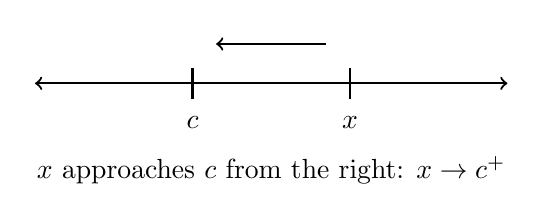
\begin{tikzpicture}
\draw[<->, thick] (-3,0) -- (3,0);
\draw[thick] (-1,-.2) -- (-1,.2); %tick mark
\draw[thick] (1,-.2) -- (1,.2);
\node[below] at (-1,-.3) {$c$};
\node[below] at (1,-.3) {$x$};
\draw[<-, thick] (-0.7,0.5) -- (0.7,0.5);
\node[below] at (0,-0.8) {$x$ approaches $c$ from the right: $x \to c^+$};
\draw[white](0, .7) -- (.1, .7);
\end{tikzpicture}
\end{center}

Note that $x \to c^+$ implies $x > c$. We refer to the limits

\[\lim_{x \to c^-} f(x)  \quad \text{and} \quad \lim_{x \to c^+} f(x) \]

as \textbf{one-sided limits}, and we refer to 

\[\lim_{x \to c} f(x) \]

as a \textbf{two-sided limit}. Note that if the associated one-sided limits are not equal, then the two-sided limit does not exist.


We can also let the inputs, $x$, either increase or decrease without bound, denoted by $x \to \infty$ and $x \to -\infty$ respectively.
These can be represented visually by the following diagrams:



\begin{center}
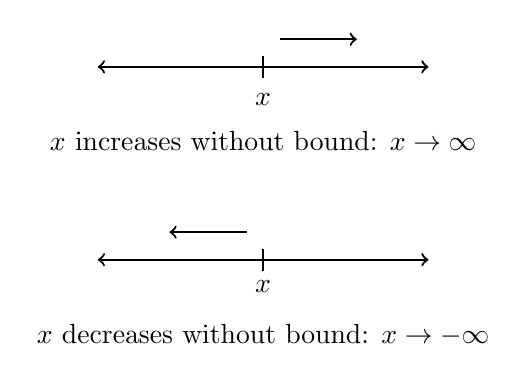
\begin{tikzpicture}[scale =0.7]
\draw[<->, thick] (-3,0) -- (3,0);
\draw[thick] (0,-.2) -- (0,.2); %tick mark
\node[below] at (0,-.3) {$x$};
\draw[->, thick] (0.3,0.5) -- (1.7,0.5);
\node[below] at (0,-1) {$x$ increases without bound: $x \to \infty$};
\draw[<->, thick] (-3,-3.5) -- (3,-3.5);
\draw[thick] (0,-3.3) -- (0,-3.7); %tick mark
\node[below] at (0,-3.7) {$x$};
\draw[<-, thick] (-1.7,-3) -- (-0.3,-3);
\node[below] at (0,-4.5) {$x$ decreases without bound: $x \to -\infty$};
\draw[white](0, .7) -- (.1, .7);
\end{tikzpicture}
\end{center}

We refer to the limits
\[\lim_{x \to \infty} f(x)  \quad \text{and} \quad \lim_{x \to -\infty} f(x) \]
as \textbf{limits at infinity}.


\section{Finding limits numerically}



In what follows, functions will be presented using formulas.  
We will determine the limit of a function by making an appropriate \textbf{table of values}.
 

\begin{example}[example 1]
Determine the following one-sided limit: 
\[\lim_{x \to 3^{+}} (x^2 + 2).\]
First,  $x \to 3^{+}$ means that $x$ is approaching the number $3$ from the right, so $x > 3$. 
To represent this numerically, consider the following values for $x$: $3.1, 3.01, 3.001, 3.0001$.
Continuing the pattern, these numbers, each greater than 3, become arbitrarily close to 3.
Now, to determine the limit numerically,  we will plug these four values of $x$ into the function $x^2 + 2$ and  
look for a pattern in the outputs.

Here is the analysis:\\
If $x = 3.1$ then $x^2 + 2 = 11.61$.\\
If $x = 3.01$ then $x^2 + 2 = 11.0601$.\\
If $x = 3.001$ then $x^2 + 2 = 11.006001$.\\
If $x = 3.0001$ then $x^2 + 2 = 11.00060001$.\\

We can summarize this information in a table:
  
%\[
%\setlength{\extrarowheight}{5pt}
%\begin{array}{ c | c | c | c | c }
%  x & 3.1 & 3.01 & 3.001 & 3.0001 \\ 
%	\hline
%	x^2 + 2 & 11.61 & 11.0601 & 11.006001 & 11.00060001
%\end{array}
%\]

\[
%\setlength{\extrarowheight}{5pt}
\begin{array}{ |c | c |}
	\hline
	x & x^2 + 2\\
	\hline
	3.1 & 11.61 \\
	\hline
	3.01 & 11.0601 \\
	\hline
	3.001 & 11.006001 \\
	\hline
	3.0001 & 11.00060001\\
	\hline
\end{array}
\]




The outputs appear to be approaching the number 11, leading us to conclude that

\[\lim_{x \to 3^+} (x^2 + 2) = 11\] 
 
In this particular example, we could have arrived at the answer by simply plugging the number $x = 3$
into the function $x^2 + 2$ since $3^2 + 2 = 11$.  
\end{example}

In general, when \textbf{plugging in} the value that $x$ is approaching yields a number, 
that number is usually the correct answer.  



\begin{problem}(problem 1)
Compute the limit by plugging in the terminal value.
\[
\lim_{x \to -4} (x^2 -3x -1)
\]

The limit is $\answer{27}$.
\end{problem}

We now turn our attention to examples where the shortcut of ``plugging in'' does not work.

\begin{example}[example 2]
Determine the following one-sided limit: $\displaystyle \lim_{x \to 1^{+}} \frac{x^3 - 1}{x^2 -1}.$\\
First, if we plug $x = 1$ into the function, we get the fraction  $\displaystyle \frac00$, which is called an \textbf{indeterminate form}. 
This means that the answer can be anything and so a deeper analysis is required.

Since $x$ is approaching $1$ from the right, we have $x > 1$. 
We can represent this numerically using the values $x =1.1, 1.01, 1.001, 1.0001$. 
To guess the limit, we will plug these values into the function $f(x) =\frac{x^3 - 1}{x^2-1}$ and  
look for a pattern in the outputs.

Here is the analysis:\\
If $x = 1.1$ then $f(x) = 1.57619$.\\
If $x = 1.01$ then $f(x) = 1.507512$.\\
If $x = 1.001$ then $f(x)= 1.500751$.\\
If $x = 1.0001$ then $f(x) = 1.5000750$.\\

We summarize this information in the table below.
  
\[
\begin{array}{|c | c|}
	\hline
  x & \frac{x^3 - 1}{x^2-1} \\
	\hline
	1.1 & 1.57619 \\
	\hline
	1.01 & 1.507512 \\
	\hline
	1.001 & 1.500751 \\
	\hline
	1.0001 & 1.500075 \\
	\hline
\end{array}
\]

The outputs appear to be approaching the number 1.5, leading us to guess that

\[\lim_{x \to 1^+} \frac{x^3 - 1}{x^2-1} = 1.5\] 
 
 In section 1.4, we will learn algebraic techniques to validate this result.
\end{example}


\begin{problem}(problem 2a)
Fill in the table below with 5 decimal places of accuracy and use it to find the limit: $\displaystyle \lim_{x \to 2^+} \frac{x^3 - 8}{x^2 - 4}$\\

\[
\begin{array}{| c | c|}
	\hline
  x & \frac{x^3 - 8}{x^2 - 4}  \\ 
	\hline 
	2.1 &  \answer{3.07561}\\
	\hline
	2.01 &  \answer{3.00751}\\
	\hline
	2.001 &  \answer{3.00075}\\
	\hline
	2.0001 &  \answer{3.00008}\\
	\hline
\end{array}
\]


Now determine the limit: $\displaystyle \lim_{x \to 2^+} \frac{x^3 - 8}{x^2 - 4} = \answer{3}$.
\end{problem}


\begin{problem}(problem 2b)
Use the table below to guess the limit: $\displaystyle \lim_{x \to 3^-} f(x)$\\

\[
\begin{array}{ |c | c|}
	\hline
  x & f(x)  \\ 
	\hline 
	2.9 &  -0.97432\\
	\hline
	2.99 &  -0.99743\\
	\hline
	2.999 &  -0.99974\\
	\hline
	2.9999 &  -0.99997\\
	\hline
\end{array}
\]

The numerical evidence suggests that the limit is: $\displaystyle \lim_{x \to 3^-} f(x) = \answer{-1}$.
\end{problem}



The next example involves both 1-sided limits and the associated 2-sided limit. 
Furthermore, the result can be interpreted as the slope of a tangent line to the graph of the exponential function $f(x) = e^x$ at $x=0$.



\begin{example}(Example 3)
Use the tables below to determine the following limits:
\[
\lim_{x \to 0^-} \frac{e^x - 1}{x}; \quad \lim_{x \to 0^+} \frac{e^x - 1}{x}; \quad\mbox{and} \quad \lim_{x \to 0} \frac{e^x - 1}{x}
\]

\[
\begin{array}{|c | c|}
	\hline
  x & \frac{e^x-1}{x}\\
  \hline
  0.1 & 1.052 \\
  \hline
  0.01 & 1.005 \\
  \hline
  0.001 & 1.0005 \\
  \hline
  0.0001 & 1.00005\\
	\hline
\end{array}
\qquad
\begin{array}{ |c | c |}
	\hline
  x & \frac{e^x - 1}{x}\\
  \hline
 -0.1 & 0.95163 \\ 
  \hline
 -0.01 & 0.99502 \\
  \hline
 -0.001 & 0.99950 \\
  \hline
 -0.0001 & 0.99995\\
 \hline
\end{array}\]

To determine the first limit, we look at the second table where $x$ is approaching $0$ from the left. 
The outputs appear to be approaching the number 1, leading us to conclude that
\[\lim_{x \to 0^-} \frac{e^x - 1}{x} = 1.\]
To determine the second limit, we look at the first table where $x$ is approaching $0$ from the right.
The outputs again appear to be approaching the number 1, leading us to conclude that
\[\lim_{x \to 0^+} \frac{e^x - 1}{x} = 1.\]
Since the one-sided limits are equal, we conclude that the two-sided limit is also equal to 1:
\[\lim_{x \to 0} \frac{e^x - 1}{x} = 1.\]
Note that the fraction $\frac{e^x - 1}{x}$ is not defined at $x=0$ since plugging in $x=0$ yields the indeterminate form $\frac{0}{0}$.
Moreover, the fraction $\frac{e^x - 1}{x}$ represents the slope of the secant line between the points $(0, e^0)$ and $(x, e^x)$ on the graph of $f(x) = e^x$.
Thus, the limit $\lim_{x \to 0} \frac{e^x - 1}{x}$ represents the slope of the tangent line to the graph of $f(x) = e^x$ at the point $(0, e^0) = (0,1)$.
\end{example}

The next problem gives the slope of the tangent line to the graph of the function $f(x) = \sin x$ at $x=0$.

\begin{problem}(problem 3a)
Fill in the missing values in the tables to 4 decimal places (make sure your calculator is in radian mode).
\[
\begin{array}{|c | c|}
	\hline
  x & \frac{\sin x}{x} \\ 
	\hline 
	0.1 & \answer{0.9983} \\ 
	\hline
	0.01 & 0.99998 \\ 
	\hline
	0.001 & 0.9999998 \\ 
	\hline
	0.0001 & 0.999999998\\
	\hline
\end{array}
\qquad
\begin{array}{|c | c|}
	\hline
  x & \frac{\sin x}{x} \\ 
	\hline 
	-0.1 & \answer{0.9983} \\ 
	\hline
	-0.01 & 0.99998 \\ 
	\hline
	-0.001 & 0.9999998 \\ 
	\hline
	-0.0001 & 0.999999998\\
	\hline
\end{array}
\]

Now use the numerical information to guess the one-sided limits:\\
$\displaystyle \lim_{x \to 0^-} \frac{\sin x}{x} = \answer{1} \quad \text{and} \quad \lim_{x \to 0^+} \frac{\sin x}{x} = \answer{1}$	\\

Based on the one-sided limits, determine the two-sided limit: $\displaystyle \lim_{x \to 0} \frac{\sin x}{x} = \answer{1}$

It should be noted that plugging $x=0$ into the 
function $\displaystyle{\frac{\sin x}{x}}$ yields the indeterminate form $\displaystyle\frac{0}{0}$, which is not a final answer.
\end{problem}

The next problem gives the slope of the tangent line to the graph natural logarithm function $f(x) = \ln x$ at $x=1$.

\begin{problem}(problem 3b)
Fill in the missing values in the tables to 3 decimal places.
\[
\begin{array}{| c | c|}
	\hline
  x & \frac{\ln(1+x)}{x}\\ 
  \hline
  0.1 & \answer{0.953}  \\ 
  \hline
	  0.01 & 0.995  \\ 
	\hline
	  0.001 & 0.9995 \\ 
	\hline
	  0.0001 & 0.99995 \\
	  \hline
\end{array}
\qquad
\begin{array}{| c | c|}
	\hline
  x & \frac{\ln(1+x)}{x}\\ 
  \hline
  -0.1 & \answer{1.054} \\ 
  \hline
	 -0.01 & 1.005 \\ 
	\hline
	 -0.001 & 1.0005 \\ 
	\hline
	  -0.0001 & 1.00005\\
	  \hline
\end{array}
\]
Now use the numerical information to guess the one-sided limits:\\
$\displaystyle \lim_{x \to 0^-} \frac{\ln(1+x)}{x} = \answer{1} \quad \text{and} \quad \lim_{x \to 0^+} \frac{\ln(1+x)}{x} = \answer{1}$	\\

Based on the one-sided limits, determine the two-sided limit: $\displaystyle \lim_{x \to 0} \frac{\ln(1+x)}{x} = \answer{1}$

It should be noted that plugging $x=0$ into the 
function $\displaystyle{\frac{\ln(1+x)}{x}}$ yields the indeterminate form $\displaystyle\frac{0}{0}$, which is not a final answer.

\end{problem}


\begin{problem}(problem 3c)
Fill in the table below with 5 decimal places of accuracy and use it to find the limit:
\[\lim_{x \to 0^+} \frac{e^{2x} - 1}{x}.\]

\[
\begin{array}{| c | c |}
	\hline
  x & \frac{e^{2x} - 1}{x}  \\ 
	\hline 
	0.1 &  \answer{2.21403}\\
	\hline
	0.01 &  \answer{2.02013}\\
	\hline
	0.001 &  \answer{2.00200}\\
	\hline
	0.0001 &  \answer{2.00020}\\
	\hline
\end{array}
\]



Now determine the limit: $\displaystyle \lim_{x \to 0^+} \frac{e^{2x} - 1}{x} =\answer{2}	$

\end{problem}







\begin{problem}(problem 3d)
Fill in the table below with 8 decimal places of accuracy and use it to find the limit: $\displaystyle \lim_{x \to 0^+} \frac{\sin 3x}{x}.$\\

\[
\begin{array}{| c | c |}
	\hline
	x& \frac{\sin 3x}{x} \\
	\hline
	0.1 & \answer{2.95520207} \\
	\hline
	0.01 & \answer{2.99955002}\\
	\hline
	0.001 & \answer{2.99999550}\\
	\hline
	0.0001 & \answer{2.99999996}\\
	\hline
\end{array}
\]

Now determine the limit: $\displaystyle \lim_{x \to 0^+} \frac{\sin 3x}{x} = \answer{3}$
\end{problem}

\begin{example}(Example 4)
Use the tables below to create limits.
\[
\begin{array}{|c|c|} 
	\hline
	x & f(x)\\
	\hline
	0.1 & 1.98523 \\
	\hline
	0.01 & 1.99852 \\
	\hline
	0.001 & 1.99985 \\
    \hline
	0.0001 & 1.99998\\
	\hline
\end{array}
\qquad
\begin{array}{|c|c|} 
	\hline
	x & f(x) \\ 
	\hline
	-0.1 & 3.14327 \\
	\hline
	-0.01 & 3.01432 \\
	\hline
	-0.001 & 3.00143 \\
	\hline
	-0.0001 & 3.00014 \\
	\hline
\end{array}
\]
The first table suggests the limit


\[
\lim_{x \to 0^+} f(x) = 2
\]

The second table suggests the limit
\[
\lim_{x \to 0-} f(x) = 3
\]

Since the one-sided limits are not equal, the two-sided limit does not exist.
we can express this by writing
\[\lim_{x \to 0} f(x) \;\; \text{DNE}.\]
\end{example}
\begin{problem}(problem 4)

Fill in the tables below with 5 decimal places of accuracy and use them to find the following limits:
\[
\lim_{x \to 0^+} f(x) \quad \text{and} \quad \lim_{x \to 0^-} f(x)
\]
\[
\begin{array}{ |c | c |}
	\hline
	x & f(x) \\ 
	\hline
	0.1 & 2.59374 \\
	\hline
	0.01 & 2.99507 \\
	\hline
	0.001 & 2.99950 \\
	\hline
	0.0001 & 2.99995\\
	\hline
\end{array}
\qquad
\begin{array}{| c | c |}
	\hline
	x & f(x) \\ 
	\hline
	-0.1 & 4.10685 \\
	\hline
	-0.01 & 4.00499 \\
	\hline
	-0.001 & 4.00050 \\
	\hline
	-0.0001 & 4.00005\\
	\hline
\end{array}
\]
Now determine the limits:\\
$\displaystyle \lim_{x \to 0^+} f(x) = \answer{3} \quad \text{and} \quad \lim_{x \to 0^-} f(x) = \answer{4}$
Since the one-sided limits are not equal, the two-sided limit does not exist.
\[\lim_{x \to 0} f(x) \;\; \text{DNE}.\]
\begin{hint}
Write DNE for does not exist.
\end{hint}
\end{problem}

\begin{example}[example 5]
Consider the limit: $\displaystyle \lim_{x \to -2^-} \frac{3}{x+2}.$\\
First, we observe that plugging in the value $x=-2$ gives $\frac{3}{0}$ which is undefined. 
Thus, we are required to make a deeper analysis to determine the limit.
Since the values of $x$ are less than $-2$, we consider values for $x$ such as 
$-2.1, -2.01, -2.001,$ and $-2.0001$ to make the following table of values:\\

\[
\begin{array}{ |c | c|}
	\hline
  x & \frac{3}{x+2}\\
  \hline
  -2.1 & -30 \\
  \hline
  -2.01 & -300 \\
  \hline
  -2.001 & -3,000 \\
  \hline
  -2.0001 & -30,000 \\
  \hline
  -2.00001 & -300,000 \\
  \hline
\end{array}
\] 

The numerical evidence suggests that as $x$ approaches $-2$ from the left, 
the values of $\frac{3}{x+2}$ are decreasing without bound. We conclude that 

\[\lim_{x \to -2^-} \frac{3}{x+2} =  -\infty \]

This result has geometric significance.
It means that the line $x=-2$ is a vertical asymptote for the graph of the equation $y = \frac{3}{x+2}.$
\end{example}



\begin{problem}(problem 5)
Fill in the table below and use it to find the limit:
\[\lim_{x \to 3^+} \frac{x}{x-3}.\]

\[
\begin{array}{ |c | c|}
	\hline
  x & \frac{x}{x-3}\\
  \hline
  3.1 & \answer{31}\\
  \hline
  3.01 & \answer{301} \\ 
  	\hline 
	3.001 & \answer{3001} \\
	\hline
	3.0001 & \answer{30001}\\
	\hline
\end{array}
\]

Now determine the limit (type infinity for $\infty$ and -infinity for $-\infty$):
\[
\lim_{x \to 3^+} \frac{x}{x-3} = \answer{\infty}
\]

\end{problem}


In the following example, we discuss limits as the input goes to $\infty$.
If $x \to \infty$ then $x$ is \textbf{increasing without bound}, and we can use very large numbers for $x$ in our table.

\begin{example}[example 6]
Consider the limit:
\[\lim_{x \to \infty} \frac{3x -2}{x + 3}. \]

Since $x \to \infty$, we will use powers of ten to generate large values of $x$ when constructing 
our table: 


\[
\begin{array}{ |c | c|}
	\hline
  x & \frac{3x -2}{x + 3}\\
  \hline
  100 & 2.8932 \\
  \hline
  1000 & 2.9890 \\
  \hline
  10000 & 2.9989 \\
  \hline
  100000 & 2.99989 \\
  \hline
  1000000 & 2.999989\\
  \hline
\end{array}
\] 

The numerical evidence suggests that as $x$ approaches $\infty$, that is, 
as $x$ increases without bound, the values of $\frac{3x -2}{x +3}$ are approaching the number $3$. Hence,
\[\lim_{x \to \infty} \frac{3x -2}{x +3} = 3. \]

This result has geometric significance.  It means that the line $y = 3$ is a horizontal 
asymptote (on the right end)for the graph of the equation $y = \frac{3x -2}{x +3}.$
\end{example}


\begin{problem}(problem 6)
Fill in the table below using \textbf{fractions} and use it to find the limit:
\[\lim_{x \to \infty} \frac{3x-2}{5x+6}.\]


\[
\begin{array}{| c | c |}
	\hline
  x & \frac{3x-2}{5x+6}\\
  \hline
  10 & \answer{28/56}  \\ 
	\hline 
	100 & \answer{298/506}\\
	\hline
	1000 & \answer{2998/5006}	\\
	\hline
	10000 & \answer{29998/50006}\\
	\hline
\end{array}
\]
Now determine the limit:
\[
\lim_{x \to \infty} \frac{3x-2}{5x+6} = \answer{3/5}
\]
This limit tells us that the line $y = \frac{3}{5}$ is a \wordChoice{
\choice{vertical}
\choice[correct]{horizontal}
}
asymptote for the graph of the equation $y = \frac{3x-2}{5x+6}$.	
\end{problem}


\section{Limits and instantaneous velocity}


\textbf{Rectilinear motion} is motion along a straight line. We will consider an object to be in motion along a number line to keep track of its location.
We let the function $s(t)$ denote the \textbf{position} of the object at time $t$. Then the displacement of the object over a time interval,
$[t_1, t_2]$ is given by $s(t_2) - s(t_1)$.  If we divide the displacement by the duration of the time interval, we get the 
\textbf{average velocity} of the object over that time interval:
\[
\text{average velocity} = \frac{s(t_2) - s(t_1)}{t_2 -t_1}.
\]


Our goal is to determine the \textbf{instantaneous velocity} of the 
object at a given time.  To do this, we will consider time intervals of shorter and shorter duration.


\begin{example}[example 7]
Suppose the position of a falling object is given by $s(t) = 100-16t^2$ where $t$ is measured in seconds and $s(t)$ is measured in feet.
Find the instantaneous velocity of the object at time $t = 2$ seconds.\\
The average velocity of the object over the time interval $[t,2]$ is given by 
\[
\text{ave vel} = \frac{s(2)-s(t)}{2-t} = \frac{36-s(t)}{2-t},
\]
since $s(2) = 100 - 16(2^2) = 36$ feet.
To obtain the instantaneous velocity, we will look for a pattern in the average velocity as the time interval $[t, 2]$ gets shorter and shorter:
\[
\begin{array}{|c | c|}
	\hline
 t & \text{ave vel}\\
 \hline
  1.9 & -62.4 \\
  \hline
  1.99 & -63.84 \\
  \hline
  1.999 & -63.984 \\
  \hline
  1.9999 & -63.9984\\
  \hline
\end{array}
\]
It appears that as the average velocities are approaching the value $-64$ ft/sec, as the time intervals 
get shorter and shorter (negative velocity just means the object is falling).  Hence, we conclude that the instantaneous velocity at time $t = 2$ seconds is $-64$ ft/sec.
Moreover, in terms of limits, the instantaneous velocity, $v(t)$, is a limit of average velocities:
\[
v(2) = \lim_{t\to 2^-} \frac{s(2) - s(t)}{2-t}.
\]
Technically, in this example we only considered the left-hand limit, $t\to 2^-$.
In the next problem, we will verify that the right-hand limit gives the same value. 
\end{example}

\begin{problem}(problem 7)
Suppose the position of a falling object is given by $s(t) = 100-16t^2$ where $t$ is measured in seconds and $s(t)$ is measured in feet.
Find the value of the limit
\[
\lim_{t\to 2^+} \frac{s(t) - s(2)}{t-2},
\]
by filling in the table below.

\[
\begin{array}{| c | c |}
	\hline
  t & \text{ave vel}\\
  \hline
  2.1 & \answer{-65.6}   \\ 
	\hline 
	 2.01 & \answer{-64.16} \\
	\hline
	 2.001 & \answer{-64.016} \\
	\hline
	 2.0001 & \answer{-64.0016}\\
	\hline
\end{array}
\]
Now determine the instantaneous velocity as a limit of the average velocities:
\[
v(2) = \lim_{t\to 2^+} \frac{s(t) - s(2)}{t-2} = \answer{-64} \text{ft/sec}.
\]


\end{problem}



\section{The Number ${\bf e}$}

The number $e$ is fundamental to calculus due to the simplicity of the calculus formulas related to the 
exponential function $e^x$ and the natural logarithm function $\ln x$. 

One origin story of this special number involves compound interest. 
Recall that the compound interest formula states that the amount of money $A$ resulting from investing a principle $P$ at an annual rate $r$ with 
the interest compounded $n$ times per year for $t$ years is given by the formula 
\[ A = P\left(1+\frac{r}{n}\right)^{nt} \]

A basic fact about compound interest is that the more frequently 
the interest is compounded, the faster the money will grow. 
To investigate this, we will focus on the variable $n$ and ask what happens as $n \to \infty.$


\begin{example}[example 8]
We will investigate the compound interest formula for the simplest possible values of $P, r$ and $t$.
Letting $P=1, r= 1$ and $t=1$ in the compound interest formula above, we get:
\[
A = \left(1 + \frac{1}{n}\right)^n.
\]
 Now, we have $A$ solely as a function of the number of compounding periods, $n$ and we can investigate the 
 effect of letting $n$ grow without bound.
 
 

Below is a table of values of $A$ corresponding to large values of $n$:


\[
\begin{array}{| c | c|}
	\hline
  n & A\\
  \hline
  10 & 2.59374 \\
  \hline
  100 & 2.70481 \\ 
	\hline 
	1000 & 2.71692\\
	\hline
	10000 & 2.71815	\\
	\hline
	100000 & 2.71827\\
	\hline
	1000000 & 2.71828\\
	\hline
\end{array}
\]

What we can see from this table is that even with the number of compounding periods being as large as 1,000,000 per year, 
the principle of \$1 will not even grow to \$3 by the end of the year.  So there appears to be a limit to the effect of increasing the 
number of compounding periods on the amount of money generated by compound interest at a rate of 100\%. 
This limit is not a simple, easily recognized number and all we can say for sure from the table is that it appears to be somewhere around 2.718.
In fact, the limit is irrational, like $\sqrt 2$ and $\pi$. The famous 18th century mathematician Leonhard Euler (1707-1783) was the first to 
refer to it as $e$, standing for ``exponential".  

In conclusion, we can define $e$ as:

\[e \equiv \lim_{n \to \infty} \left(1+\frac{1}{n}\right)^n \]


To fifteen decimal places Euler's number is:

\[ e = 2.718281828459045... \]

\end{example}




\begin{problem}(problem 8)
Fill in the table below with 5 decimal places of accuracy and use it to find the limit:
\[\lim_{n \to -\infty} \left(1+\frac{1}{n}\right)^n.\]


\[
\begin{array}{| c | c|}
	\hline
  n & \left(1+\frac{1}{n}\right)^n\\
  \hline
  -100 & \answer{2.73200}   \\ 
	\hline 
	-1000 & \answer{2.71964} \\
	\hline
	-10,000 & \answer{2.71842}	\\
	\hline
	-100,000 & \answer{2.71830}\\
	\hline
\end{array}
\]

Now determine the limit (the answer is a well known number, denoted by a single letter):
\[
\lim_{n \to -\infty} (1+\frac{1}{n})^n = \answer{e}
\]
\end{problem}




\begin{center}
\begin{foldable}
\unfoldable{Here is a detailed, lecture style video on numerical limits:}
\youtube{YX-gSPKPCTU}
\end{foldable}
\end{center}




\end{document}





